\section{Recurrent networks and sequences}

\begin{frame}{Sequences} 
	%\begin{columns}
	%	\begin{column}{.5\textwidth}
			\begin{itemize}
				\item Natural language tasks 
				\item Event processing  
				\item Statefull systems in general
			\end{itemize}	
	%	\end{column}
	%	\begin{column}{.5\textwidth}
		\begin{block}{Types}
			\begin{itemize}
				\item Variable length sequences, all elements known ahead of time. 
				\item Constant length sequences, all elements known ahead of time. 
				\item Constant length sequences, revealed one element at a time.
				\item Variable length sequences, revealed one element at a time.
			\end{itemize}
		\end{block}

	%	\end{column}
	%\end{columns}
\end{frame}

\begin{frame}{Functions of form $y_t = f(y_{t-1}, x_t; \theta)$}

\begin{eqnarray}
I_t =& UX+Vh_{t-1}+b \\
h_t =& tanh(I_t) \\
O_t =& Wh_t + c 
\end{eqnarray}

\begin{center}
\begin{figure}
	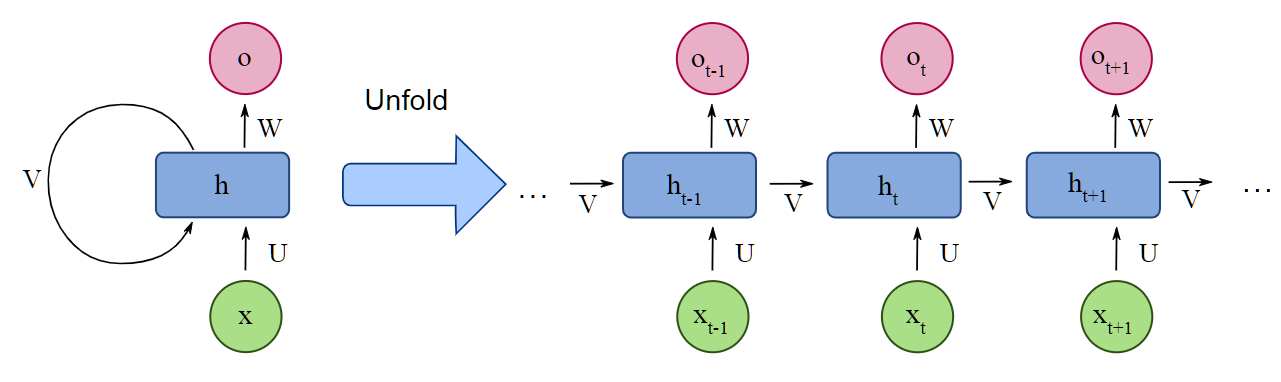
\includegraphics[width=.8\textwidth]{figures/rnn_wikipedia_1}
	\caption*{\tiny{"Recurrent neural network" (2020) Wikipedia. Available at:
	https://en.wikipedia.org/wiki/Recurrent\_neural\_network}}
\end{figure}
\end{center}
\end{frame}

\begin{frame}{Recurrent network architecture styles}
\begin{center}
	\begin{figure}
		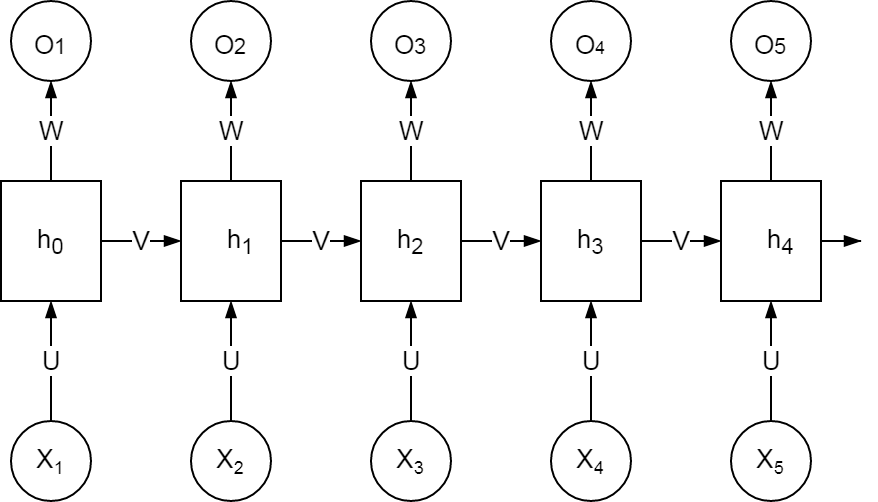
\includegraphics[width=1\textwidth]{figures/rnn_seq_2_seq}
		\caption*{{Sequence to sequence network}}
	\end{figure}
\end{center}
\end{frame}
\begin{frame}{Recurrent network architecture styles}
\begin{center}
	\begin{figure}
		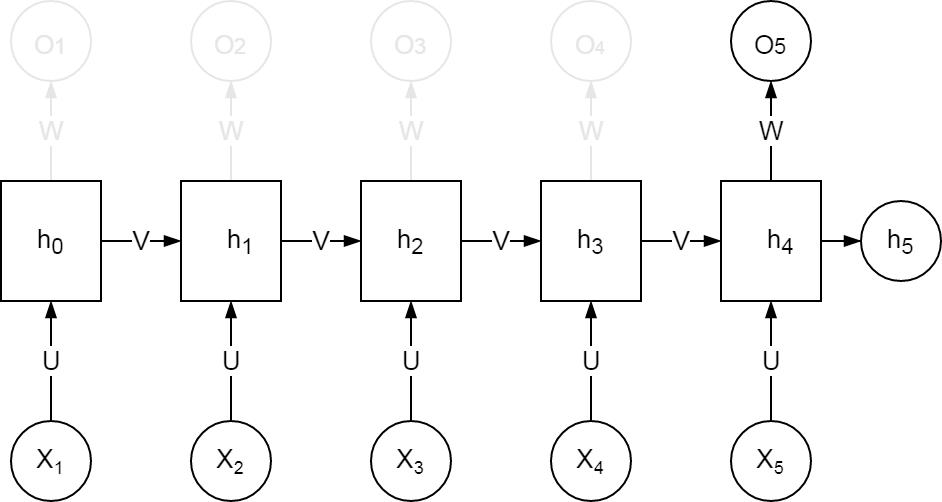
\includegraphics[width=1\textwidth]{figures/rnn_seq_2_vec}
		\caption*{{Sequence to vector network}}
	\end{figure}
\end{center}
\end{frame}
\begin{frame}{Recurrent network architecture styles}
\begin{center}
	\begin{figure}
		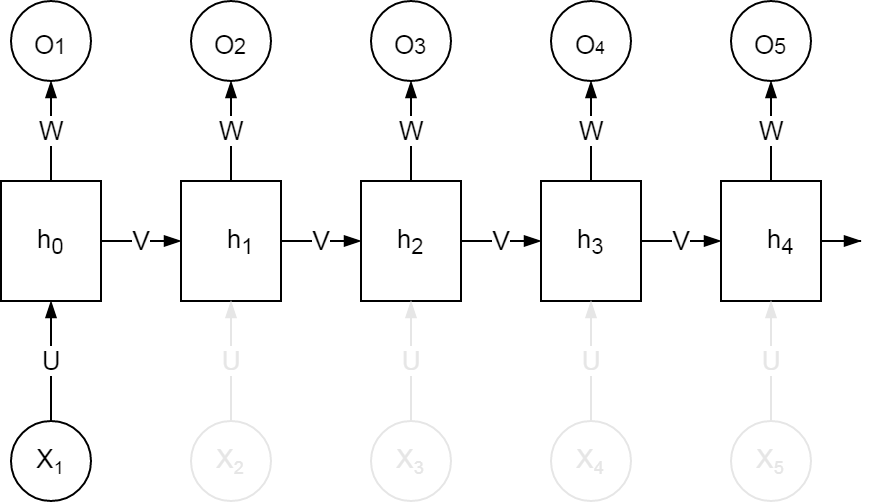
\includegraphics[width=1\textwidth]{figures/rnn_vec_2_seq}
		\caption*{{Vector to sequence network}}
	\end{figure}
\end{center}
\end{frame}
\begin{frame}{Recurrent network architecture styles}
\begin{center}
	\begin{figure}
		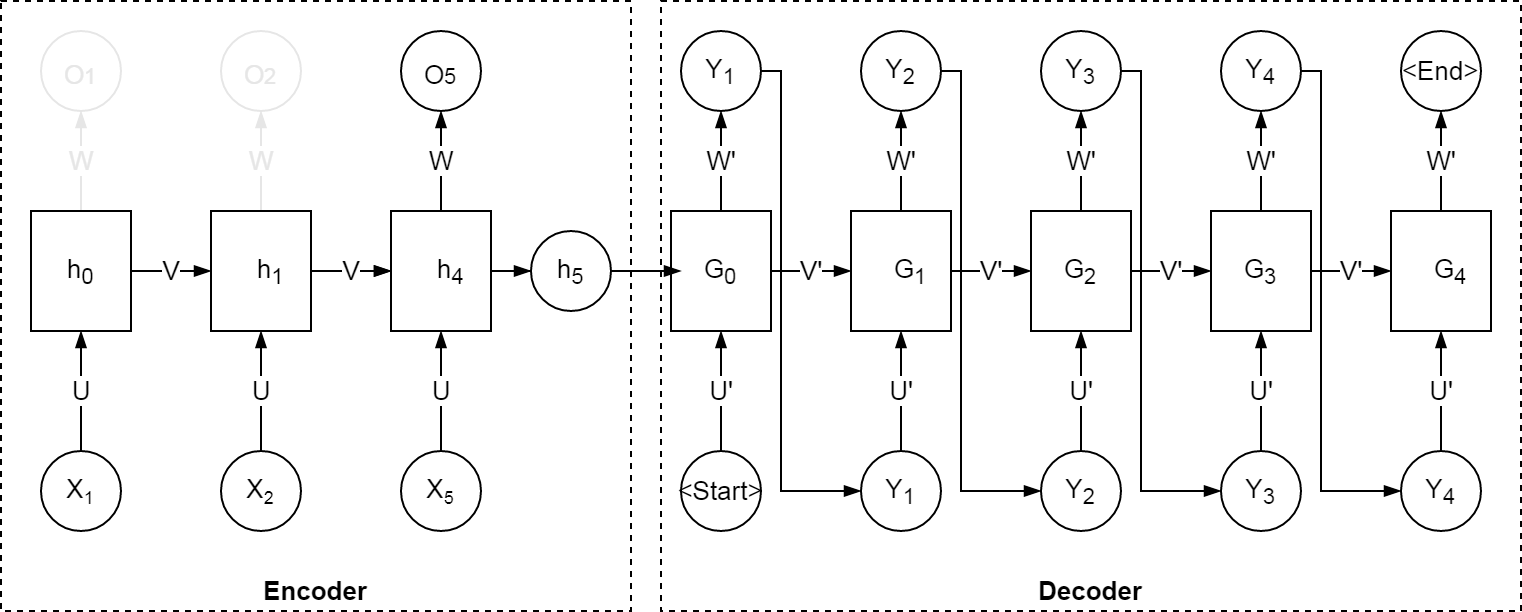
\includegraphics[width=1\textwidth]{figures/rnn_seq_2_seq_encoder_decoder}
		\caption*{{Sequence to sequence encoder-decoder network}}
	\end{figure}
\end{center}
\end{frame}